\documentclass[a4paper,twocolumn]{article}
\usepackage[utf8]{inputenc}
\usepackage[T1]{fontenc}
\usepackage{graphicx}
\usepackage{amsmath}
\usepackage{hyperref}
\usepackage{enumitem}
\usepackage{geometry}
\geometry{margin=1.2cm}
\usepackage{fancyhdr}
\usepackage{titlesec}
\usepackage{multicol}
\usepackage{parskip}
\usepackage{indentfirst}
\setlength{\columnsep}{0.6cm} % Space between columns
\setlength{\columnseprule}{0.4pt} % Vertical rule between columns

\title{Semester Project Report\\
Approximating Images with Rectangles using Simulated Annealing
}
\author{
Student Name: Maksym Khavil\\
Username: khavimak
}
\date{\today}

\begin{document}
\maketitle

\section*{1. Project Assignment}

I have chosen custom assingment of "painting from rectangles" inspired by the article "Paintings-from-Polygons: Simulated Annealing". Dahmani and others used polygons to draw pictures by optimizing mean square differnce of painted triangles and "painted" image using Simulated Annealing. I have chosen to work with rectangles with strictly horizontal or vertical sides due to ease of implementation and in attempt to try different approach towards the problem.

\section*{2. Problem Analysis}

Problem is given by a raster image with three 8 bit channels and a number of rectangles that could be placed on a canvas, if a pixel is not covered by any of rectangles it is set to be pitch black (zeros for each RGB value).
Quick calculation shows that each pixel lies in space with $255 ^ 3 = 16'581'375$ points, every rastor image can be represented as a pixel tuple of size $w \cdot h$, where $w$ is width and $h$ is height of the image.
For example marvellous picture of a smile with resolution of $128 \times 128$ lies in space with $10^{11.43}$ states. Real images with greater resolution must be embedded into even larger spaces.

\section*{3. Method Selection}

I have tried to use classical Simulated Annealing for smiley (1st image on figure 1) and it converged to unspoken digital horror (2nd image on figure 1) after running for 3 hours on my PC.

\begin{figure}[h!]
        \centering
        \begin{minipage}[t]{0.08\textwidth}
                \centering
                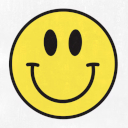
\includegraphics[width=\linewidth]{data/smiley.jpg}
        \end{minipage} \label{fig:sbs-1}
        \begin{minipage}[t]{0.08\textwidth}
                \centering
                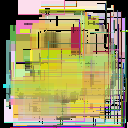
\includegraphics[width=\linewidth]{data/test1.png}
        \end{minipage}
        \begin{minipage}[t]{0.08\textwidth}
                \centering
                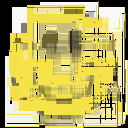
\includegraphics[width=\linewidth]{approx/smiley-gg.png}
        \end{minipage}
        \caption{Comparison of outputs during optimization.}
        \label{fig:sidebyside}
\end{figure}

Hence I have tried to shrink state space. The biggest factor in this product is all possible colors, that pixel can be. So I have decided to use only those that are present in image. It is done by sampling $k$ random points from image, then during annealing rectangles can be colored only by those colors. This approach yielded 3rd image on figure 1. All pictures in this report use $k=32$ samples.

\section*{4. Method Application}

Running algorithm on other pictures gave intereseting results. Here are approximations of Mondrian's Composition, Van Gogh's Starry Night and Da Vinci's Mona Lisa.

\begin{figure}[h!]
        \centering
        \begin{minipage}[t]{0.16\textwidth}
                \centering
                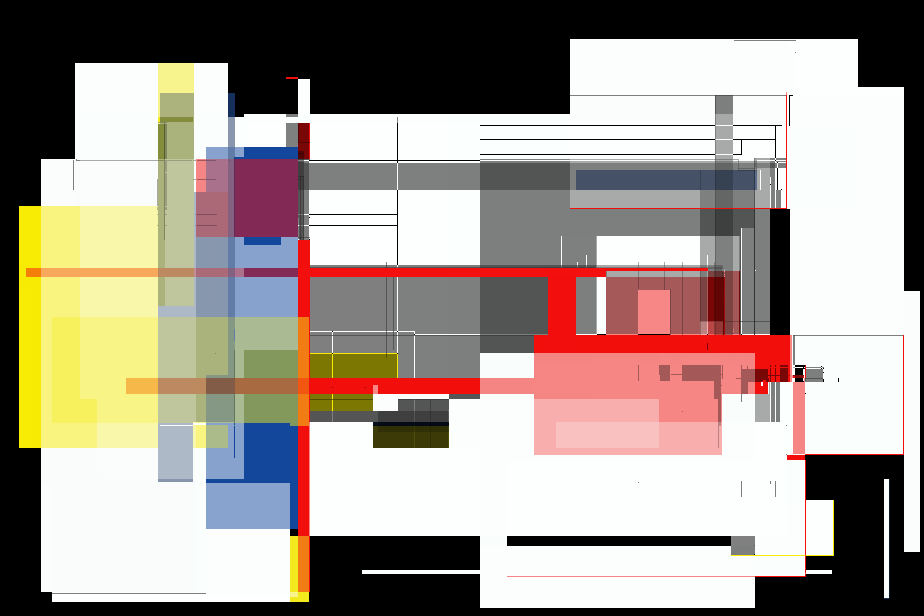
\includegraphics[width=\linewidth]{approx/piet_mondrian_composition.png}
        \end{minipage}
        \begin{minipage}[t]{0.14\textwidth}
                \centering
                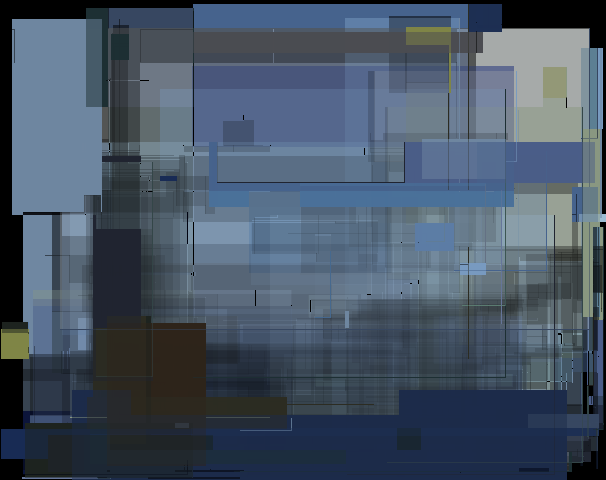
\includegraphics[width=\linewidth]{approx/van_gogh_starry_night.png}
        \end{minipage}
        \begin{minipage}[t]{0.08\textwidth}
                \centering
                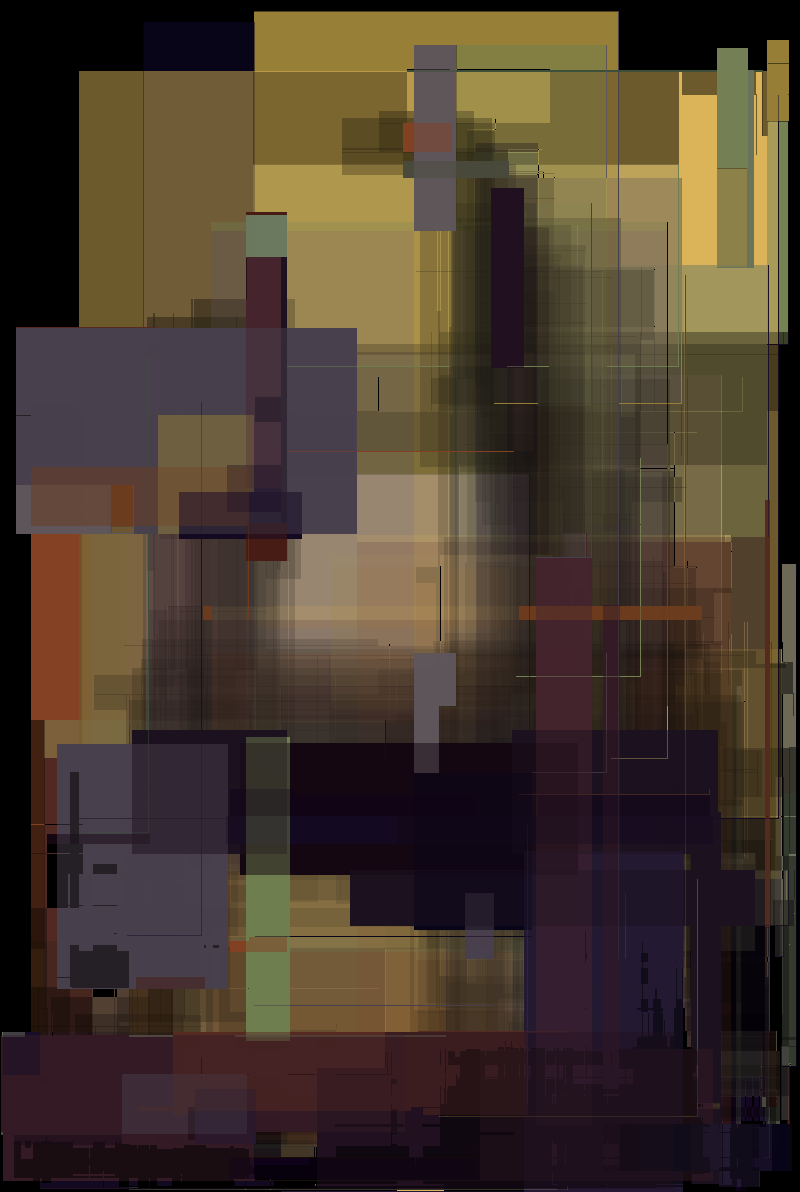
\includegraphics[width=\linewidth]{approx/davinci_monalisa.png}
        \end{minipage}
        \caption{Comparison of outputs during optimization.}
        \label{fig:sidebyside}
\end{figure}

It is easy to see how poor is the first and relative success of the last two. My hypothesis is that both smiley and Composition use sharp edges and raw colors, that are hard to hit correctly and are sensetive to minor changes in color, whereas Mona Lisa and Starry Night are more forgiving both for human eyes and algorithm.

\section*{4. Implementation}

This tool is implemented in C++ with CLI interface, instructions for which can be found in README. Makefile was chosen to be build system of this project and clang++ is used for compilation and linking.

Implementation uses \href{https://github.com/nothings/stb?tab=readme-ov-file}{stb} library for image loading and saving. Algorithm and neighbouring (mutation) schema - changing either color or only one side of the rectangle and calculating change only over changed region - proved to be very fast on small images, like smiley, but took ages on images of larger resolution, so my implementation supports multithreading for constructing neighbors.

In annealing cycle three instances of candidates are hold, the best, keeping lowest mean square error, current, which is changed in every iteration descibed by schema above, than its MSE is compared with previous. Algorithm always accepts better candidate and stochastically based on temperature may not reject worse solution.

\section*{5. References}

\begin{itemize}[leftmargin=1cm]
        \item \href{https://ceur-ws.org/Vol-2827/KBS-Paper\_2.pdf}{Paintings-from-Polygons: Simulated Annealing} by Redouane Dahmani, Sven Boogmans, Arne Meijs and Daan van den Berg
\end{itemize}

\end{document}
